\scanpage{107}
\mspage{106}%
de Hodge), et par la condition que l'on a
\[
i_2=\overset{\handwritten{\rule{0.8em}{0.4pt}}}{i_1}\quad\text{i.e.}\quad i_2(\handwritten{\lambda})=\overset{\handwritten{\rule{2.2em}{0.4pt}}}{i_1(\handwritten{\bar{\lambda}}\rlap{\tikz[baseline=0pt,x=1em,y=1em]{\draw (-.05,.25)--(.65,.25);}})}\quad\text{pour tout}\quad\handwritten{\lambda\in}\underline{C}.
\]

Si à toute variété projective lisse $X$ sur $\underline{C}$ on associe sa cohomologie rationelle $H^{\unsure{*|'}}(X,\underline{Q})=V$, de sorte que $V_{\underline{C}}=H^*(X,\underline{C})$ est isomorphe canoniquement (par la théorie de Hodge) à $H_{\mathrm{Hdg}}(X)=\handwritten{\coprod}H^q(X,\handwritten{\underline{\Omega}}^p_{X/\underline{C}})$, on voit qu'on trouve ainsi une pré-structure de Hodge sur $H^{\handwritten{*}}(X,\underline{Q})$, d'où un \inserted{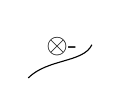
\begin{tikzpicture}[baseline=-.2ex,x=1em,y=1em]
\node[anchor=base west] at (0,.4) {$\otimes$-};
\draw (-.3,-.5) .. controls (.4,.2) and (1.7,.05) .. (2,.7);
\end{tikzpicture}}foncteur naturel de la catégorie des motifs sur $\underline{C}$ dans la catégorie des pré-s\rlap{c}t\rlap{t}r\unsure{\rlap{r}u|u}ctures de Hodge. La conjecture de Hodge \unsure{stándart|standart} équivaut à dire que ce foncteur est \uline{pleinement fidèle}, i.e. que l\deleted{e}'homomorphisme naturel qui va du groupe de Galois de Hodge précédent $G$ dans le groupe de Galois motivique (associé au \inserted{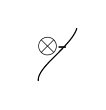
\begin{tikzpicture}[baseline=-.2ex,x=1em,y=1em]
\node[anchor=base west] at (0,.4) {$\otimes$-};
\draw (.4,-.6) .. controls (.35,-.1) and (1.6,.65) .. (1.8,1.3);
\end{tikzpicture}}foncteur de Betti $H_{\mathrm{Bet}}$) est un épimorphisme. O\rlap{\raisebox{.6ex}{U}}u encore que pour toute catégorie 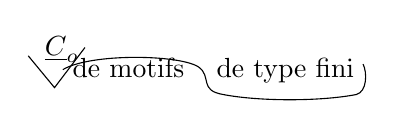
\begin{tikzpicture}[baseline=0pt,x=1em,y=1em]
\node[anchor=base west] at (0,.8) {\inserted{$\underline{C}_o$}};
\node[anchor=base west] at (1,0) {de motifs};
\node[anchor=base west] at (6.2,0) {\inserted{de type fini}};
\draw (-.25,.8)--(.7,-.35)--(1.8,1.1);
\draw (1,.3) .. controls (2,.9) and (5.2,.85) .. (5.9,.4) .. controls (6.4,.05) and (5.9,-.45) .. (6.8,-.6) .. controls (8.1,-.85) and (10.3,-.85) .. (11.6,-.6) .. controls (12,-.5) and (12,.2) .. (11.85,.5);
\end{tikzpicture} sur $\underline{C}$, désignant par $\underline{C}$ la \inserted{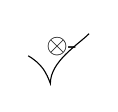
\begin{tikzpicture}[baseline=-.2ex,x=1em,y=1em]
\node[anchor=base west] at (0,.4) {$\otimes$-};
\draw (-.3,.3) .. controls (.2,0) and (.35,-.3) .. (.5,-.7) .. controls (.5,.1) and (1.5,.7) .. (1.9,1.1);
\end{tikzpicture}}catégorie de pré-s\unsure{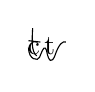
\begin{tikzpicture}[baseline=0pt,x=1em,y=1em]
\node[anchor=base west,inner sep=0pt] at (0,0) {c};
\node[anchor=base west,inner sep=0pt] at (.6,0) {t};
\draw (.2,.95) .. controls (.18,.55) and (.14,.1) .. (.35,-.05);
\draw (.05,.5)--(.48,.45);
\draw (.05,.25) .. controls (.05,-.2) and (.4,-.25) .. (.45,-.1) .. controls (.6,.3) and (.65,.3) .. (.7,.15) .. controls (.78,-.3) and (.9,-.3) .. (1,-.05) .. controls (1.15,.4) and (1.3,.5) .. (1.4,.45);
\end{tikzpicture}}ructures de Hodge engendrée par \deleted{celle-ci,} les $H_{\mathrm{Bet}}(M)$ pour $M\handwritten{\in}\operatorname{Ob}(\underline{C}_o)$, l'homomorphisme de groupes algébriques $G\handwritten{\longrightarrow}G_o$ associé au foncteur de Betti-Hodge $\underline{C}_o\handwritten{\longrightarrow}\underline{C}$ est un épimorphisme (i.e. surjectif sur les points à valeurs complexes, disons).


O\rlap{\raisebox{-.6em}{\handwritten{n}}}n appelle \deleted{structure} \uline{polarisation} d'une pré-structure de Hodge de poids $n$ la donnée d'un accouplement de préstructures de Hodge
\[
\handwritten{\phi}:V\mathbin{\mathrm{x}}V\handwritten{\longrightarrow}\underline{Q}(n),
\]
où $\underline{Q}(n)$ est l'espace vectoriel trivial $\underline{Q}$ sur $\underline{Q}$, avec $\underline{Q}_{\underline{C}}=\underline{C}$ muni d\rlap{e}u \deleted{la} bidegré $(n,n)$), ayant la propriété que la forme hermitienne correspondante sur $V_{\underline{\mathbb{C}}}$,
\margin{\handwritten{\unsure{
\begin{tikzpicture}[baseline=0pt,x=1em,y=1em,rotate=25]
\draw (0,0) .. controls (.15,.2) and (.35,.5) .. (.45,.8) .. controls (.3,.2) and (.1,-.15) .. (0,0);
\draw (.25,.6)--(.42,.4)--(.8,.9)--(.48,.2)--(.7,.35)--(1.15,.8) .. controls (1,.4) and (.7,0) .. (.95,.05) -- (1.8,.35);
\draw (1.1,.4) .. controls (1.1,.75) and (1.4,.7) .. (1.5,.4) .. controls (1.65,.4) and (1.68,.72) .. (1.8,.5);
\draw (.05,-.3)--(2,-.3);
\end{tikzpicture}|$\psi$|$\phi$}}}
\[
\handwritten{\psi}(x,y)=\handwritten{\phi}(x,\overset{\handwritten{\rule{0.5em}{0.4pt}}}{y})(\handwritten{\unsure{i|-i}})^{p\handwritten{-q}}\quad\text{pour }x\text{ de bidegré }(p,\deleted{\unsure{n}}\handwritten{q}\unsure{-}p)
\]
soit définie positive. U\rlap{\tikz[baseline=0pt,x=1em,y=1em]{
\draw (.1,.95) .. controls (.08,.75) and (.12,.65) .. (.27,.65);
\draw (.45,1) .. controls (.45,.8) and (.55,.7) .. (.7,.9);
\draw (.55,.7)--(.62,.6);
}}ne \uline{structure de Hodge} est une préstructure de Hodge admettant une polarisation. Les structures de Hodge forment une \margin{\tikz[baseline=0pt,x=1em,y=1em]{\draw (0,0)--(.13,.12)--(.2,.3);}}sous-$\otimes$-catégorie de la catégorie des pré-structures de Hodge. La théorie de Hodge nous assure que le foncteur de Betti-Hodge sur la catégorie des

